\chapter{Introduction}
\label{chapter:Introduction}
\thispagestyle{myheadings}

\graphicspath{{1_Intro/Figures/}}

\section{Motivation}
\label{sec:history}

From speech production to athletic performance, implementing reproducible motor gestures is integral to expressing meaningful actions. While it is clearly important to have the ability to execute  learned skills with high precision, often over the timescales of years, it is not clear how centrally controlled motor systems maintain this ability. A simple theory is that the individual neurons involved are as stable as the motor skill itself, where reproducible actions result from stereotyped patterns of neural activity. However, it is clear that we rely on external feedback to guide learned skills. Neurons must somehow acclimate to changes in our behavioral state and environment to produce desired motor outputs. These conditions can vary greatly, even over the course of hours, suggesting that individual neurons may need to significantly change their firing properties over these timescales to produce the same motor output. Neuronal circuits must constantly evaluate the tradeoffs between stable operating regimes and plastic adaptation to changing environmental demands. This balancing act is not trivial. In most cases, individual neurons remain physically integrated with surrounding circuitry for several decades. While it is clear that axons and dendrites can be highly dynamic even in adult animals \cite{Holtmaat2009-ie}, it is not clear to what extent individual neurons maintain stable activity patterns over extended time periods in the face of changing environmental demands.
 
Even given constant environmental conditions it is not clear how reproducible the timing and participation of cells in central motor networks are when performing the same action. In fact, the stability of neural tuning for motor systems is not necessarily expected.  Vast numbers of neurons in motor cortex converge to relatively few muscles, suggesting that a given muscular activation pattern could be produced by many, potentially redundant, patterns of neural activity. In parallel, single neurons in motor cortex have been shown to switch tuning properties in a task-dependent manner \cite{Koralek2012-nd}. While the production of stereotyped movements is important for many motor tasks, it is equally critical to maintain the ability to flexibly adapt this motor plan in response to changing environmental conditions to achive dynamic motor objectives. 
 
Neurophysiological evidence suggests that at a mesoscopic scale, neural populations exhibit similar activity patterns over time. In mice, surface cortical layers maintain heterogeneous, log-normally distributed firing rates that remain largely stable across learning \cite{Barth2012-bu}. Sensory cortical areas contain sparsely active neurons interspersed within networks of largely unresponsive cells \cite{Hromadka2008-uv} \cite{Lefort2009-ne}  \cite{Yassin2010-if} and this functional architecture is largely preserved over days to weeks \cite{Margolis2012-pt}, although it is unclear what mechanisms direct these embedded cells \cite{Hromadka2008-uv}. In the hippocampus, earlier electrophysiological methods tracking tens of cells emphasized stable neural tuning over a timescale of a week, whereas recent studies tracking thousands of cells using new optical techniques revealed that $75-85\%$ of the cells change their tuning properties within the same timeframe (Ziv et al. 2013). In the whisker motor cortex, individual neurons in mice trained on an object detection task were not active reliably, but the relationship between ensemble measurements and behavior remained stable \cite{Huber2012-hf}. These studies support the view that for stable behaviors, individual neurons involved can show substantial changes in participation.
 
Adaptive neural tuning is likely driven by homeostatic processes- neurons retain a tendency toward a relatively stable equilibrium between competing interdependent network elements \cite{Turrigiano2008-hq} . Homeostatic tuning has been observed in vivo, particularly in the visual system using chronic multielectrode recordings to monitor firing rates in the visual cortex of freely behaving rats during chronic monocular visual deprivation \cite{Hengen2013-js} \cite{Mrsic-Flogel2007-ed}. Similar tuning has been seen in the Barrel cortex \cite{Holtmaat2009-ie} and hippocampus  \cite{Hirase2001-ow} \cite{Goold2010-fb}. Intriguingly, it seems as though much of these homeostatic processes are occurring over periods of sleep \cite{Hengen2013-js} \cite{Mrsic-Flogel2007-ed} \cite{Hengen2016-nw}.
 
To address how motor networks achieve stable behavioral outputs, it is critical that we study an experimentally tractable animal model that can learn to produce stereotyped motor sequences. Invertebrates such as the larval zebrafish present an appealing model, given recent advances in volumetric video-rate imaging of calcium dynamics in large numbers of neurons during fictive swimming  \cite{Ahrens2012-nu}. Yet, it is not clear if larval zebrafish are capable of more complex motor behaviors. Rodents produce stereotyped sequences in their grooming rituals \cite{Colonnese1996-bi} and to a certain extent their overall behavioral performance \cite{Wiltschko2015-hz}. However, these grooming rituals and behavioral gestures remain challenging to quantify \cite{Wiltschko2015-hz}. While rodents produce ultrasonic vocalizations that are easy to quantify, \cite{Holy2005-jv} it is unclear if ultrasonic vocalizations are learned or even centrally controlled. One promising alternative is to study skilled reaches in mice \cite{Azim2014-te}. Unfortunately, for all of these behaviors, the central motor circuits underlying each behavior remain undefined. 
 
Songbirds present a unique opportunity to study the neural mechanisms underling learned, stereotyped motor sequences. Birdsong is an easily quantifiable sequential behavior that is both learned and reproducible on a millisecond time-scale. Zebra finches recapitulate the same song for years \cite{Lombardino2000-cb}  and the neural circuitry that produces song is extremely well studied and well-defined \cite{Nottebohm1976-hv} \cite{Nottebohm1976-bq}

Even when environmental conditions and behavioral performance variability are constrained, questions about coding spatiotemporal organization and stability at the single neuron level have been notoriously difficult to address given the technical challenge of stably recording from single neurons over timescales relevant for learning. A major push in this thesis is to develop technologies to maintain chronic recordings of the same neurons over days.  I will describe devices developed for extracellular recordings \emph{(Chapter 2)} and for  optical imaging of genetically encoded calcium indicators \emph{(Chapter 3)} as well as their deployment to study a  behavior that is well-constrained and preserved for years \emph{(Chapter 4 \& Chapter 5)}. Using these techniques, we have been able to offer insights that reconcile these apparently contradictory views on motor tuning. Our experimental evidence suggests that the brain encodes learned behaviors coarsely at a mesoscopic level that is highly stable, but individual neurons embedded within these networks can change their firing patterns. Possibly, the stability of a memory may be rooted in the robustness of network patterns, where single neurons can adapt to optimize motor output. 


\section{Research outline}

This thesis is divided into two parts of approximately equal length. The first part describes the development and deployment of new tools to study motor stability in awake, behaving animals. The second section focuses on the characterization of mesoscopic and fine scale network dynamics of the song premotor cortical zone HVC ( used here as a proper name) in zebra finches through in vivo electrophysiology and calcium imaging. 
 
\textbf{PART 1:} \textit{Engineering tools for long term neural recording in small animals }

\begin{itemize}
	\item \textbf{Chapter 2} discusses the development of the carbon fiber electrode array that enabled the experiments described in \emph{Chapter 4 \& Chapter 5}. The array is comprised of a 16 channels that self-splay upon entering the brain like the bristles of a paintbrush, providing densely sampled recordings with  a minimally invasive interface. 
		
	\item \textbf{Chapter 3} discusses the development of a 3D printed, wireless capable miniature microscope for single-photon fluorescence imaging in freely behaving animals, that enabled  experiments described in \emph{Chapter 5}. The device is made from 3D printed parts and off-the-shelf components. These microscopes weigh less than 2g, can be configured to image a variety of fluorophores, and can be used wirelessly or in conjunction with active commutators. Microscope control software, based in Swift for macOS, provides low-latency image processing capabilities for closed-loop, or BMI, experiments.
	\end{itemize}


\textbf{PART 2:} \textit{Systems level description of HVC dynamics}

\begin{itemize}
	\item \textbf{Chapter 4}  describes a series of experiments where we recorded both single units and local field potentials (LFPs) in the freely behaving zebra finch using self-splaying carbon fiber electrodes and miniature head-mounted microscopes. We reveal that excitatory and inhibitory neurons were entrained to opposite phases of a prominent 30Hz LFP, and that nearby projection neurons are active close in time,  strongly suggesting that local inhibition gates excitatory neuron firing.

	\item  \textbf{Chapter 5} describes that in the song  premotor nucleus, HVC, mesoscopic patterns of inhibition are stable for months, but that interspersed populations of projection neurons coding for song can change from day to day. The most dramatic shifts occur over intervals of sleep. In contrast to the transient participation of excitatory neurons, ensemble measurements dominated by inhibition persist unchanged even after damage to downstream motor nerves. These observations offer a principle of motor stability: spatiotemporal patterns of inhibition can maintain a stable scaffold for motor dynamics while the population of principal neurons that directly drive behavior shift from one day to the next.

	\item Finally, I conclude with a discussion of future directions based on these experiments in \textbf{Chapter 6}.
		
	\end{itemize}


\section{Background}


\subsection{ General Motor Learning/ Maintenance}

Successful sensorimotor learning depends on the generation of a skilled motor behavior that consistently yields outcomes that are expected or favorable. Motor skill learning is canonically defined as the repetitive, trial-and-error process used to form and increase the speed and accuracy of a new motor behavior \cite{Diedrichsen2015-zc}  \cite{Shmuelof2014-xs} \cite{Shmuelof2014-tn}. Learning a new motor skill begins with a rapid initial improvement followed by more moderate refinements over a longer time period \cite{Karni1998-mu}. The early stages involve exploration of a range of behaviors and outcome-based evaluation and selection.  Later in the learning process, repetition-based refinements of the task dominate, driving the formation of a highly stereotyped movement with minimal trial-to-trial variability. 

The process of updating a system by reinforcing internal states that led to favorable outcomes is a fundamental tenant of reinforcement learning \cite{Kaelbling1996-op} \cite{Andrew1998-kn} \cite{Sutton1998-bp}. Framing neurobiological learning in this computational framework has contributed greatly to understanding how biological networks process information \cite{Niv2009-qd}  and, in turn, these studies have inspired algorithms for machine learning \cite{Sutton1998-bp}. Reinforcement learning explicitly requires exploration. The network probes the consequences of various actions and registers or updates their values. This process allows the network to adaptively and contextually regulate the expression of the probed actions. There is increasing evidence that the brain implements computations predicted by reinforcement learning theory \cite{Daw2006-jd}  \cite{Niv2009-qd} \cite{Eshel2015-qd}  \cite{Schultz1997-vh}.
 
Neuronal circuits have to achieve an ongoing trade-off between attempts to achieve stable operating regimes while evaluating and updating output in order to retain plasticity mechanisms for adapting to changing environmental demands. A critical step in addressing the detailed biological mechanisms in reinforcement learning is to have a well constrained behavior that naturally converges around a set point, where stability in light of environmental challenges is actively maintained. 

\subsection{Zebra Finch Song Behavior}


Songbirds present themselves as an excellent model to study the neural activity that produces stable behavior. While the vocal repertoire of the zebra finch is diverse and complex \cite{Woolley2005-of}, the stereotypical male courtship song provides a unique opportunity for reproducible hypothesis testing, making it one of  the most studied and best understood models for motor learning \cite{Williams2004-hn}. The neural circuits that underlie song behavior are well defined, extensively studied, and in key respects homologous to the cortico-basal ganglia circuits underlying sensory-motor learning in mammals. 

\begin{figure}[!htb]
 %\begin{minipage}[t]{0.49\linewidth}\centering
    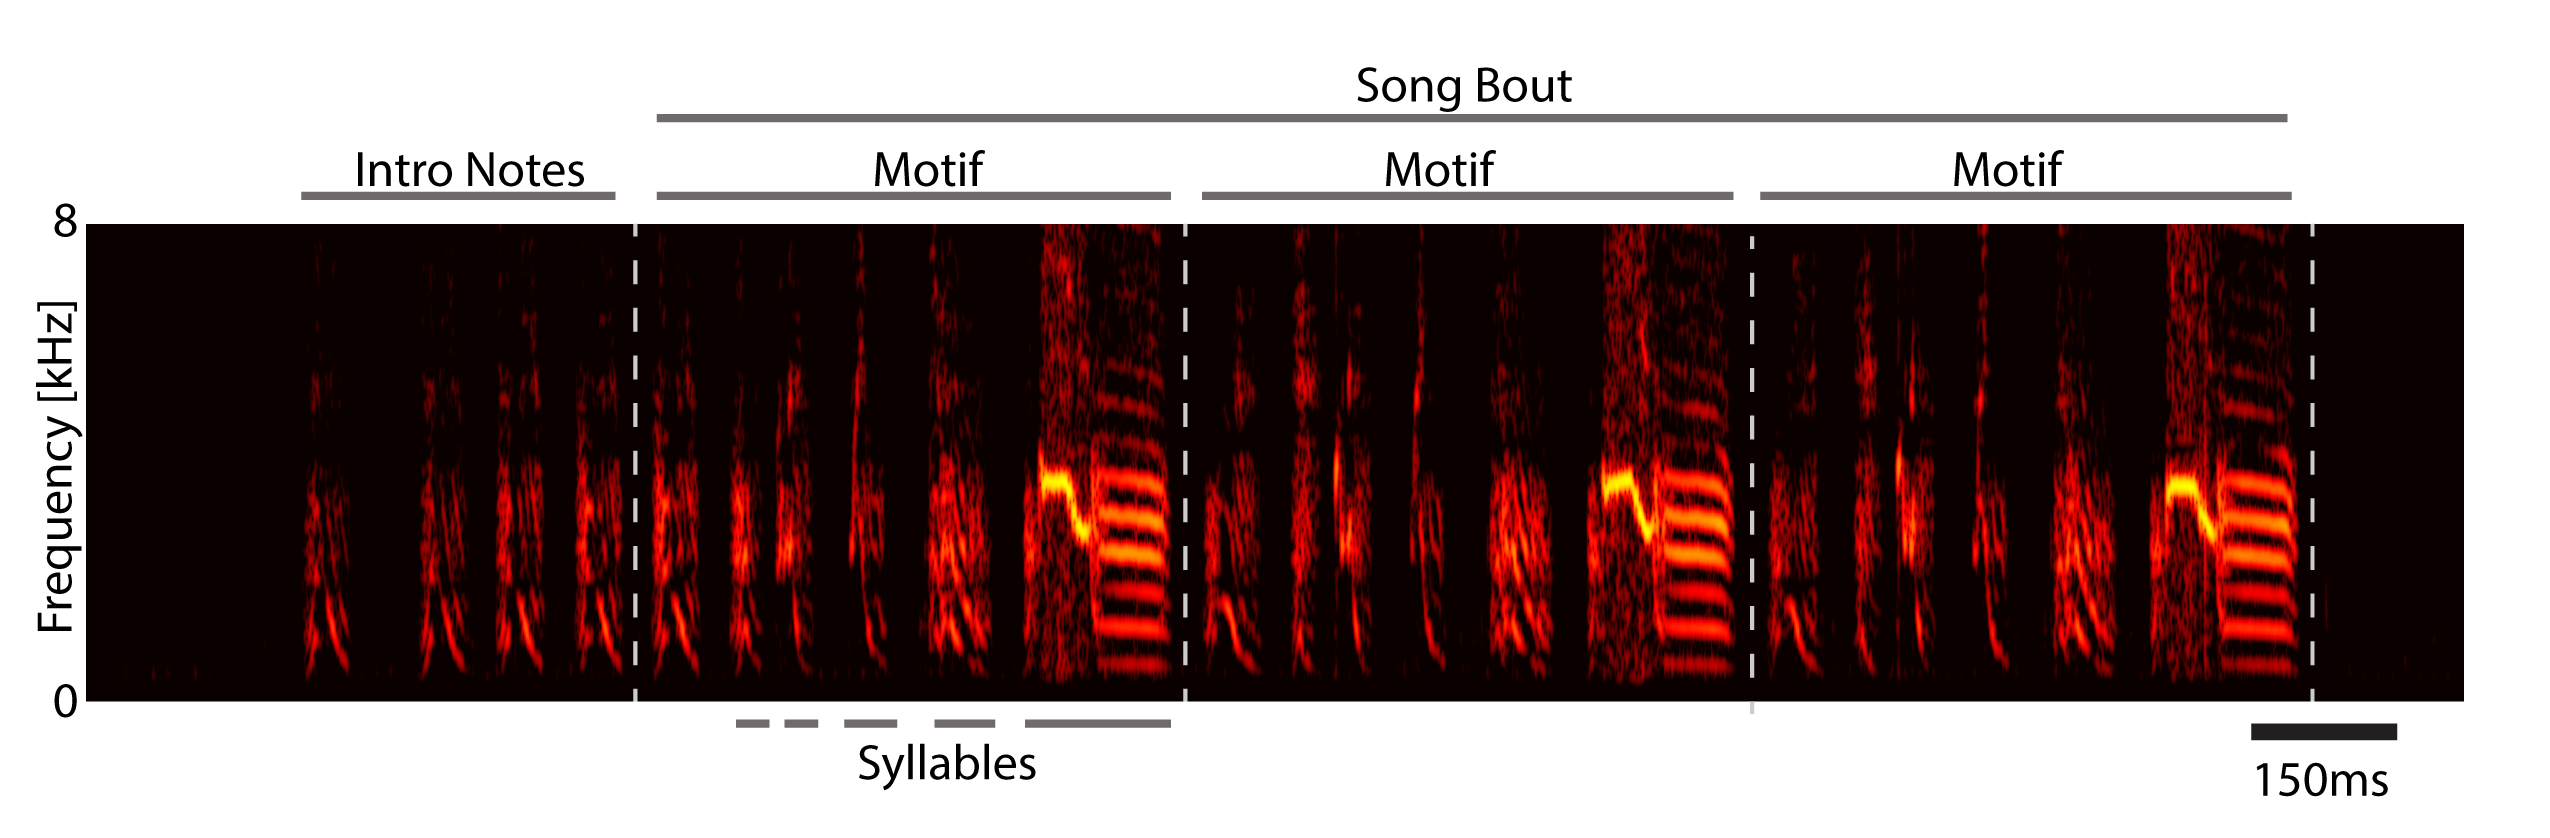
\includegraphics[width=15cm]{figure1.png}
    \centering
\medskip
\caption[Song structure of the male zebra finch]{\footnotesize  \textbf{Song structure of the male zebra finch} Spectrogram demonstrating the behavior of the adult male zebra finch songbird, including the song bout, and its comprising motifs. Each motif, in turn, is comprised of vocal elements called syllables. }

\label{fig:Sampling}
\end{figure}

For the male zebra finch, singing behavior is a complex, learned, stereotyped motor action that is behaviorally relevant, and, once learned, is performed with great precision. Each song bout consists of many repetitions of a canonical or dominant motif that spans 0.5-1 seconds \cite{Williams2004-hn} with an occasional minor variation \cite{Sossinka1980-lf}. Adult finches will produce hundreds and thousands of motifs per hour in isolation \cite{Pytte2011-pb}. A motif is then comprised of 3-7 smaller vocal elements called syllables that range from tens to hundreds of milliseconds in duration, and each syllable is highly stereotyped \cite{Glaze2006-rl}. The stereotyped nature and repetition frequency of zebra finch song make them  well-suited for the study of sequential motor behaviors.
					
The zebra finch is considered a \emph{closed-ended learner}, which means that they do not learn new vocal elements after the first 90 days after hatching, the period of flexible vocal exploration \cite{Funabiki2009-ah}. However, adult zebra finches do retain some plasticity in adulthood, and they are able to modify both the spectral and the temporal characteristics of individual syllables, but only to a limited extent. Finches can learn to change features of their song in response to experimentally-delivered conditional auditory feedback (CAF) \cite{Ali2013-db} \cite{Andalman2009-lj}. Additionally, the stereotopy and spectral structure of song degrades significantly after deafening in the adult, an effect that is reversed by lesions of the basal ganglia \cite{Brainard2001-ep} \cite{Hamaguchi2014-sx}. Interestingly, there is a dramatic change in variability when zebra finches direct their songs to females. Even in juveniles, the presence of a female leads to a sharp reduction in spectral variability and duration \cite{Aronov2012-jj} \cite{Kojima2011-wy}. A possible mechanisms for this effect is a reduction of variability in spiking in the song motor circuit involved in trial and error learning. \cite{Hessler1999-bo}  \cite{Kao2006-gp}.

\subsection{ Song Circuit overview}

\begin{figure}[!htb]
 %\begin{minipage}[t]{0.49\linewidth}\centering
    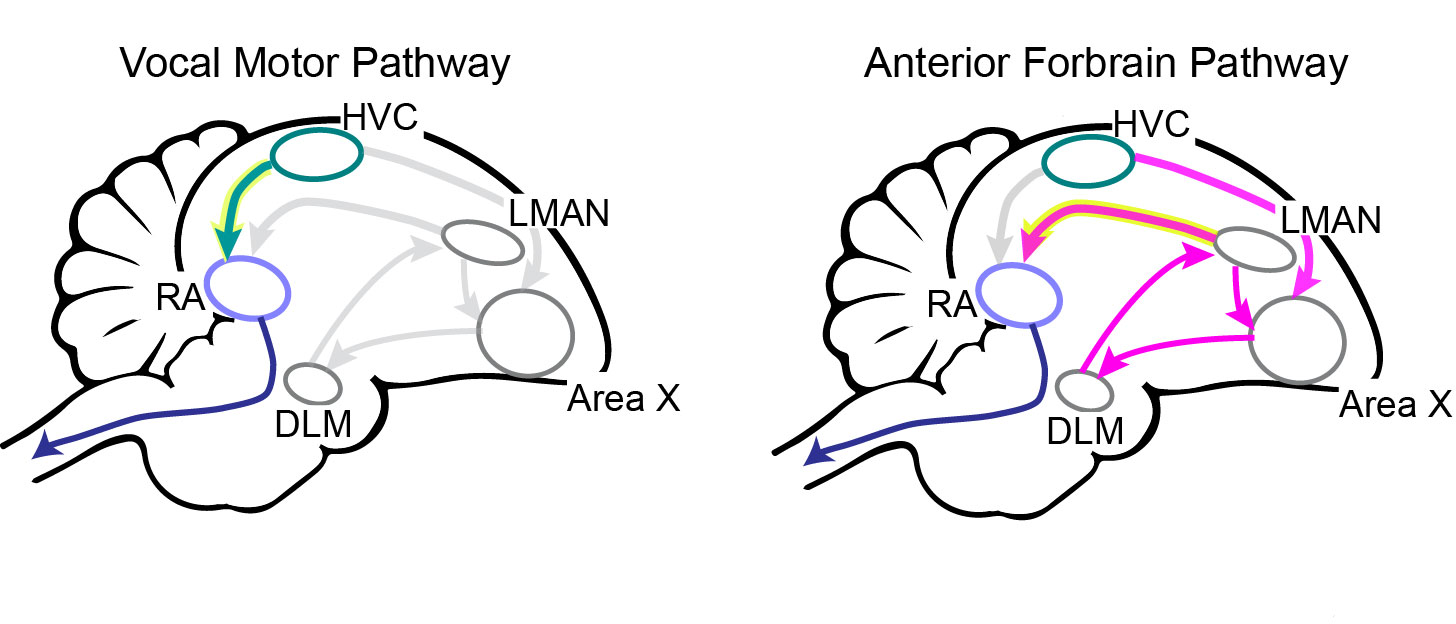
\includegraphics[width=14cm]{figure2.jpg}
    \centering
\medskip
\caption[Song circuit overview]{\footnotesize  \textbf{Song circuit overview.} \textbf{a}, \textit{Left,} Vocal Motor Pathway \textbf{(VMP)}, which acts as a simple motor hierarchy.  \textit{Right,} the Anterior Forebrain Pathway \textbf{(AFP)}, which is involved in trial-and error vocal learning.  It is important to note that both pathways include the nuclei HVC and RA.}

\label{fig:Sampling}
\end{figure}


The neural circuitry underlying the zebra finch's song is one of the best described in neuroscience. This circuit is distributed throughout the brain in small computational engines called \emph{nuclei}, that are distributed into two primary pathways: the\emph{ vocal motor pathway} (VMP) that mediates adult, stereotyped vocal performance, and the \emph{anterior forebrain pathway} (AFP) that underlies vocal exploration and learning \cite{Aronov2008-kx} \cite{Olveczky2005-mc}. Of critical interest are two nuclei. The first is the premotor nucleus,\emph{ HVC}, which is the shared origin of the VMP and the AFP. The second is the \emph{robust nucleus of the arcopallium} (RA), a critical component of the descending motor pathway where both the VMP and the AFP converge. From RA, neurons project to the hypoglossal nucleus \emph{nXII}, in the brainstem and neurons in the caudal portion of nXII directly innervate the muscles controlling the syrinx \cite{Olveczky2005-mc} \cite{Vicario1988-dl}. RA has a weak projection to the nXII and another projection to brainstem nuclei that controls breathing \cite{Sturdy2003-ed} \cite{Krutzfeldt2004-po}. Both pathways are described in some detail below. 


\subsection{Vocal Motor pathway	}

At the apex of the VMP, there is a strong non-topographic projection from HVC to RA (Foster and Bottjer, 1998). Physiological evidence suggests that HVC neurons projecting to RA (HVC$_{RA}$) provide temporal control of song through addressing disparate, discrete locations within RA. In turn, different RA neurons innervate different muscle groups in the bird's vocal organ \cite{Fee2011-en}. Supporting this, unilateral lesions of RA in the adult result in severe deficits in vocal production (Ashmore et al., 2008), whereas unilateral lesions of HVC mostly affect song sequencing \cite{Williams2004-hn}. This effect is relatively subtle compared to bilateral lesions that cause adults to revert to juvenile-like subsong \cite{Aronov2008-kx}. A one-to-many projection from HVC to RA would allow individual HVC$_{RA}$ neuron bursts to coordinate the activity of multiple muscles at a single point in time. In this way, the VMP is simply a motor control hierarchy.


\subsection{Anterior Forebrain Pathway (AFP)}

Anatomically, in the AFP, projection neurons begin in HVC, which sends axons to the striatopallidal nucleus \emph{Area X}. This area shares strong physiological similarities to the mammalian basal ganglia \cite{Goldberg2010-fm}  \cite{Fee2011-en}. Pallidal neurons in Area X project to the dorsolateral division of the medial thalamus (DLM). DLM, in turn, projects to LMAN, which sends bifurcating axon collaterals to both RA and back to Area X \cite{Nixdorf-Bergweiler1995-nj}  \cite{Vates1995-zr}. Lesions of LMAN or Area X have not been shown to have a pronounced effect on the structure or timing of adult song \cite{Olveczky2005-mc} (Scharff and Nottebohm, 1991) (Sohrabji et al., 1990). However, lesions of either DLM or LMAN in juveniles and adults result in a significant decrease in trial-to-trial song variability and song stereotypy increases \cite{Aronov2008-kx}  \cite{Fee2011-en} \cite{Kao2006-gp}  \cite{Olveczky2005-mc}. Alternatively, bilateral lesions of HVC in adult birds leads to a regression of song to a state that resembles juvenile-like babbling \cite{Aronov2008-kx} . Together, these results suggest that the AFP, specifically the LMAN $\rightarrow$ RA projections, provides a source of trial and error variability, where the evaluation of this variation could form the basis of trial and error learning. Still, the basic mechanisms of how the AFP injects noise into RA, and how beneficial noise is incorporated into the VMP, remain to be directly observed. 
 
These theories have been tested explicitly in studies where the bird must shift the pitch of a targeted syllable to avoid playback of aversive white noise \cite{Andalman2009-lj} \cite{Tumer2007-oj}. If the AFP is inactivated after multiple days of learning, the pitch will revert back to the outcome of the previous day's learning. \cite{Tumer2007-oj} This observation strongly implies that the AFP rapidly generates fluctuations to explore advantageous variations and mediates fast learning and that VMP learns new motor programs slowly, potentially over periods of sleep \cite{Andalman2009-lj}.  


\subsection{HVC physiology}

Projection neurons in HVC can be broadly classified by their downstream projection targets, including basal ganglia-projecting neurons (HVC$_{X}$) that project to the AFP and are thought to be involved in trial-and-error learning and motor projecting neurons (HVC$_{RA}$), which in turn project to brainstem respiratory and vocal nuclei that directly drive the vocal organ \cite{Krutzfeldt2004-po}. A third, much larger projection neuron type that innervates the auditory region avalanche (HVC$_{AV}$) also sparsely populates the nucleus.
Individual HVC neurons fire a brief, 10ms volley of action potentials (where firing rates can exceed 100Hz!) at the same point in a song over many repetitions \cite{McCasland1987-cf}, sparsely coding for points in time throughout the song. \cite{Hahnloser2002-nl}. HVC$_{RA}$ neurons burst at a single point in a song with < 1ms onset jitter between repetitions of the same song. HVC$_{X}$ cells appear to share the same sparse coding properties of HVC$_{RA}$ neurons, though they tend to burst more than once per motif \cite{Kozhevnikov2007-jz}. HVC$_{I}$ neurons produce dense, complex, repeating patterns. Given that the downstream neurons in RA burst at many points throughout the song \cite{Leonardo2005-up}, it has been proposed that there is a many-to-one projection from HVC$_{RA}$ neurons. This convergence would allow single HVC$_{RA}$ neurons to act as the ticks of a clock with each 'tick' triggering the recruitment of multiple muscle groups as needed throughout the song.
 
Mild cooling of HVC with a bilaterally implanted Peltier device results in linear stretching of spectral components of a song, whereas cooling of RA does not affect song timing, suggesting that the neural dynamics generated by intrinsic circuitry within HVC controls moment-to-moment timings of acoustic features in the syllables of adult song. \cite{Long2008-go}  \cite{Fee2011-vs}. Also, dense sampling of projection neurons reveals largely uniform coverage in time \cite{Picardo2016-tj} \cite{Hahnloser2002-nl}). These results have suggested that a ballistic propagation of synaptically connected premotor neurons in HVC form a synaptic chain that forms a basic clock, dictating song timing in a top-down manner. 
However, direct excitatory synapses are sparse \cite{Kornfeld2017-lq} and excitatory neuron coupling is low \cite{Mooney2005-ev}. Moreover, it is clear that inhibition plays a large role in coordinating and stabilizing these dynamics \cite{Markowitz2013-ly}.

In a closely related species, the bengalese finch, cooling HVC alters the transition probabilities between syllables, reducing the number of repetitions of long-repeated syllables and increases the randomness of syllable sequences. In addition, HVC neurons in this species that project to the basal ganglia (HVC$_{X}$) display context-dependent activity correlated to syllable repetition and transition \cite{Wang2008-ml}. Additionally, in finches, stimulation of HVC during singing can terminate, restart, or rearrange song syntax \cite{Vu1998-gz}  \cite{Wang2008-ml}. Furthermore, UVA, an upstream input to HVC, displayed activity locked to the offsets of song motifs and song bouts. Taken together, this evidence suggests that timing and probabilistic sequencing of motor action can share the same localized neural circuit within HVC and that it can be influenced by its upstream inputs. 
 
	
Previous studies of HVC have only characterized the activity of small numbers of single neurons recorded serially \cite{Hahnloser2002-nl} \cite{Kozhevnikov2007-jz} Long et al., 2010; Yu and Margoliash, 1996). Until the work described in this thesis, no group has directly observed the relationship between single cells and network activity during the production of song. Rectifying the mismatch between models describing HVC dynamics and the lack of experimental data to validate them is a critical aim of this thesis. Even now, we are still only taking the first steps toward a long journey of understanding HVC at single cell resolution, and on a network scale. For example, basic questions about network function, such as how and to what degree the stability of neuronal activity is balanced with plasticity in brain circuitry, has been largely ignored- primarily because addressing these challenges requires longitudinal measurements from the same neurons in vivo, which has been difficult to achieve using classical neurophysiological techniques. The work described in the following chapters only scratches at the surface of these mysteries. 




%%%%=========[ Extra crap ===========%%



%\bigskip

%{\it Consider the following Java-JDT plugin name in German: "`Plugin-Entwicklungsumgebung"'.}

%\bigskip

%Clearly, this is a problem, and BU librarians will complain. One way of fixing
%this issue is to enclose the offending paragraph in {\tt
%	$\backslash$begin\{sloppypar\}} and {\tt $\backslash$end\{sloppypar\}},
%resulting in the following outcome:

%\bigskip

%\begin{sloppypar}
%	{\it Consider the following Java-JDT plugin name in German:
%		"`Plugin-Entwicklungsumgebung"'.}
%\end{sloppypar}

%\bigskip

%Indeed, although the paragraph spacing becomes sloppy, at least you can hand in
%the thesis!


%LaTeX has a steep learning curve. You can use the original book by Lamport to
%learn more \cite{lamport1985:latex}, but there are many on-line resources with
%excellent instructions and examples. Just Google a LaTeX topic you would like to
%explore.

%As far as editing and compilation of LaTeX sources, if you have not found one
%yet, TexStudio seems to be quite popular.

